\documentclass{jsarticle}
\usepackage{moreverb}
\usepackage[dvipdfmx]{graphicx, hyperref}
\usepackage{float}
\usepackage{amsmath}
\usepackage{amssymb}

\usepackage{atbegshi}
\ifnum 42146=\euc"A4A2 \AtBeginShipoutFirst{\special{pdf:tounicode EUC-UCS2}}\else
\AtBeginShipoutFirst{\special{pdf:tounicode 90ms-RKSJ-UCS2}}\fi

\bibliographystyle{junsrt}


\title{計算機実習 問題14.12 成長する表面}
\author{早稲田大学先進理工学部物理学科 B4 藤本將太郎}
\date{\today}

\begin{document}
\maketitle
    
\section{シミュレーションの目的}
    表面科学における問題の1つは粗い表面の形成を理解することにある.$t=0$で平らな表面があったとする.蒸着や沈着の結果として表面がどのように成長するかを考えてみよう.たとえば,初め直線上に並んだ$L$個の占有された格子点があるとする.成長は垂直な方向に制限されている(図14.13参照).以前と同様に,周辺の点をランダムに選んでそれを占有する.クラスターの平均の高さは
    \begin{equation}
        \bar{h} = \frac{1}{N_{s}}\sum_{i=1}^{N_{s}}h_{i}
    \end{equation}
    で与えられる.ここで$h_{i}$は基線から$i$番目の表面の点までの距離である.和はすべての表面の点$N_{s}$個についてとられる(イーデン・モデルにおける表面の点の正確な定義は問題14.12で議論されている).
    
    粒子1個が付着するたびに$t$を1だけ増加させる.ここでの主な興味は表面の”幅”が$t$とともにどのように変化するかにある.表面の幅を
    \begin{equation}
        \omega^{2} = \frac{1}{N_{s}}\sum_{i=1}^{N_{s}}(h_{i}-\bar{h})^{2}
    \end{equation}
    で定義する.一般に,表面の幅$\omega$は$L$と$t$に依存し,表面の粗さの尺度を与える.初め$\omega$は時間とともに大きくなり,
    \begin{equation}
        \omega(L,t) \sim t^{\beta}
    \end{equation}
    であると予想される.指数$\beta$は垂直方向に沿った成長の時間相関を記述する.図14.13はイーデン・モデルによる表面の発展を示している.ある特徴的な時間の後のゆらぎが相関している長さが$L$と同じ程度になり,幅は$L$のみに依存する定常な値に達する.つまり,
    \begin{equation}
        \omega(L, t \gg 1) \sim L^{\alpha}
        \label{eq:14-12-e2}
    \end{equation}
    である.$\alpha$は粗さ指数として知られている.
    
    式(\ref{eq:14-12-e2})からは,定常状態では基線に垂直方向の表面の幅は$L^{\alpha}$で成長することが分かる.このような幅についての定常状態の振る舞いは自己アフィンフラクタルの特徴の1つである.そのようなフラクタルは異方的なスケール,すなわち,異なる方向で異なる長さのスケールをもつ場合の変換のもとで(平均として)不変である.例として,表面を水平方向に因子$b$でスケールし直すとしよう.このとき,もとの表面とスケールされた表面とが相似性を保つためには表面の垂直方向を因子$b^{\alpha}$でスケールし直さなければならない.
    
    短い長さのスケール,つまり,界面の幅よりも短い長さでは,表面は荒れていてその粗さは指数$\alpha$で特徴づけられる(表面を歩く蟻を想像せよ).しかし,表面の幅よりもずっと長いスケールでは,表面は平らに見えるようになり,ここの例では,一次元的になる.問題14.12では,いくつかの成長モデルで与えられる表面の特性が調べられる.

\section{作成したプログラム}
    本シミュレーションで作成したプログラムを以下に示す。


    \subsection{イーデン・モデルに基づき界面の成長を記述するプログラム}
    このプログラムは,3つのクラスからなる.今回のシミュレーションのコアであるクラスEdenと,パラメータ等の設定ダイアログの表示を行うクラスTopWindow,そのダイアログでボタンを押した際に実行される関数群をまとめたものであるクラスMainである.プログラムを実行すると,まずMainが呼び出され,その初期化関数\_\_init\_\_の中でTopWindowが呼び出され,ダイアログが表示される.ボタンを押すと,それに対応するMain内の関数が実行され,結果を得ることができる.
    Edenにおいて,ウィンドウの縦の長さを決めるために,問題cで確認されたスケーリングの関係と,イーデン・モデルのクラスターのフラクタル次元がおよそ2であることを用いている(29行目).また,glow\_latticeの中では時間の経過ごとに最大の高さを検出して,随時格子の大きさを変化させることによって,どれだけ長い時間シミュレーションを行っても良いようにしてある(初めから大きなサイズの配列をつくろうとするとエラーとなる).基本的な成長規則はイーデン・モデルのシミュレーションで過去に行ったものと同じである.また,描画に関しては,内容が更新された格子のみを描画更新するようにしてある.しかし,このように描画を行うと,最終的に得られた図が,保存した時に汚くなることがあったので,最後のステップの終了後,一旦全てのキャンバス内のオブジェクトを削除して初期化してから,もう一度全体を描画するようにした.アニメーションや表面サイトの強調表示はオプションで変更することができる.問題b,cの実行は長時間の試行を繰り返すものであるので,時間がかかることを注意しておく.
       \listinginput{1}{14-12_growing_surface.py}
        
\section{実習課題}

    \begin{enumerate}
        \renewcommand{\labelenumi}{\alph{enumi}.}
        \renewcommand{\labelenumii}{}
        
        \item \textbf{イーデン・モデル}.イーデン・モデルでは,周辺の点がランダムに選ばれ占有される.このモデルでは,”オーバーハング”が存在し得る.また,高さ$h_{x}$は基線から列$x$における周辺の点までの距離の中で最大のものに対応する.水平方向に周期的境界条件を用いてすべての周辺の点を定めよ.成長の規則は通常のイーデン・モデルと同様であるが,成長は長さ$L$の帯の上端から始まる.$L=100$の正方格子を調べ,表面の成長とともに表面のようすがどのように変化していくか述べよ.表面を明確に定めることができるか.周辺の点の多くはどこにあるか.周辺の点の部分集合として表面の点が定義されている(すなわち,ある$x$に対して最大の$h$を持つ点).もし全ての周辺の点を含めたら,結果は定性的に異なると考えるか.
            \begin{enumerate}
                \item $L=100$の正方格子で,表面の成長とともに表面の様子がどのように変化していくのかを観察した.実際に得られた図を図\ref{fig:14-12-f1}に示した.このとき,黒で示した部分は占有された格子点を表し,水色で示した部分は周辺の点,赤色で示した部分は周辺の点のうち,ある$x$に対して最大の$h$を持つ点,すなわち表面の点を表している.
                
                \begin{figure}[H]
                    \begin{center}
                        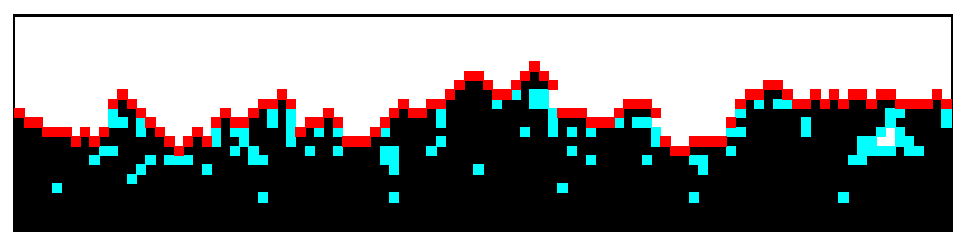
\includegraphics[width=10.0cm]{figure_1.pdf}
                        \caption{$L=100$のとき,成長させて得られた表面の様子}
                        \label{fig:14-12-f1}
                    \end{center}
                \end{figure}
                図\ref{fig:14-12-f1}から,周辺の点の多くは表面の近くに存在していることが分かる.また,成長に応じて,成長したクラスターの表面の幅(赤色の部分の分布の偏差)は大きくなっていくことが観察される.具体的にどのように変化しているかについては,問題bで確かめることとする.
            \end{enumerate}
        
            
        \item 同じグラフ上に,$L=32, 64, 128$について幅$\omega(t)$を時間の関数としてプロットし,イーデン・モデルの指数$\alpha$と$\beta$の値を求めよ.どのようにプロットするのが最も適当か.幅は初めべき乗則にしたがって成長するか.もしそうであるなら指数$\beta$を求めよ.その時間の後に表面の幅が定常状態の値となるような,$L$に依存するクロスオーバ時間はあるか.どのようにして$\alpha$の値を得ることができるか.数値的に得られている$\beta$と$\alpha$の最も良い値は,それぞれに対して予言されている正確な値$\beta=1/3$,$\alpha=1/2$と一致している.

            \begin{enumerate}
                \item 同じグラフ上に$L=32,64, 128$について幅$\omega(t)$を時間の関数として,両対数グラフにしてプロットした(図\ref{fig:14-12-f2}).このとき,これらの値は15回の試行の平均をとったものとなっている.
                \begin{figure}[H]
                    \begin{center}
                        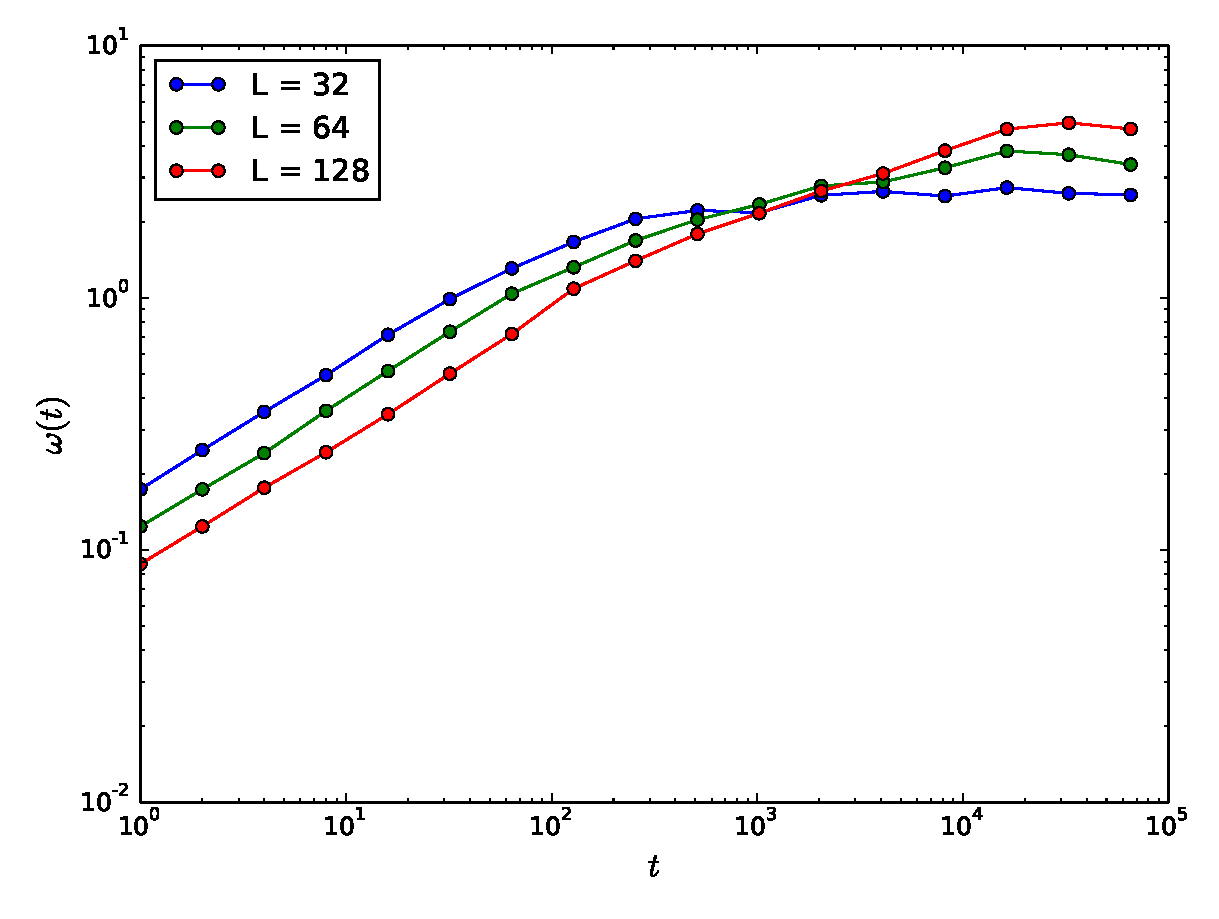
\includegraphics[width=10.0cm]{figure_2.pdf}
                        \caption{$L=32,64,128$について幅$\omega(t)$を時間$t$の関数として両対数グラフにしたもの($T\sim 100000$).}
                        \label{fig:14-12-f2}
                    \end{center}
                \end{figure}
                このようにすると,幅$\omega$は初め両対数グラフ上で直線に乗るので,ベキ乗則に従うことがわかる.このとき,
                \begin{equation}
                    \omega(L,t) \sim t^{\beta}
                \end{equation}
                として$L=128$の場合について$\beta$を求めると,$\beta=0.508658$となる.また,他の$L$に関しても$\beta$の値は同じであることが確かめられる.しかし,これは理論的に予測されている値$\beta=1/3$とは異なっている.
                \begin{figure}[H]
                    \begin{center}
                        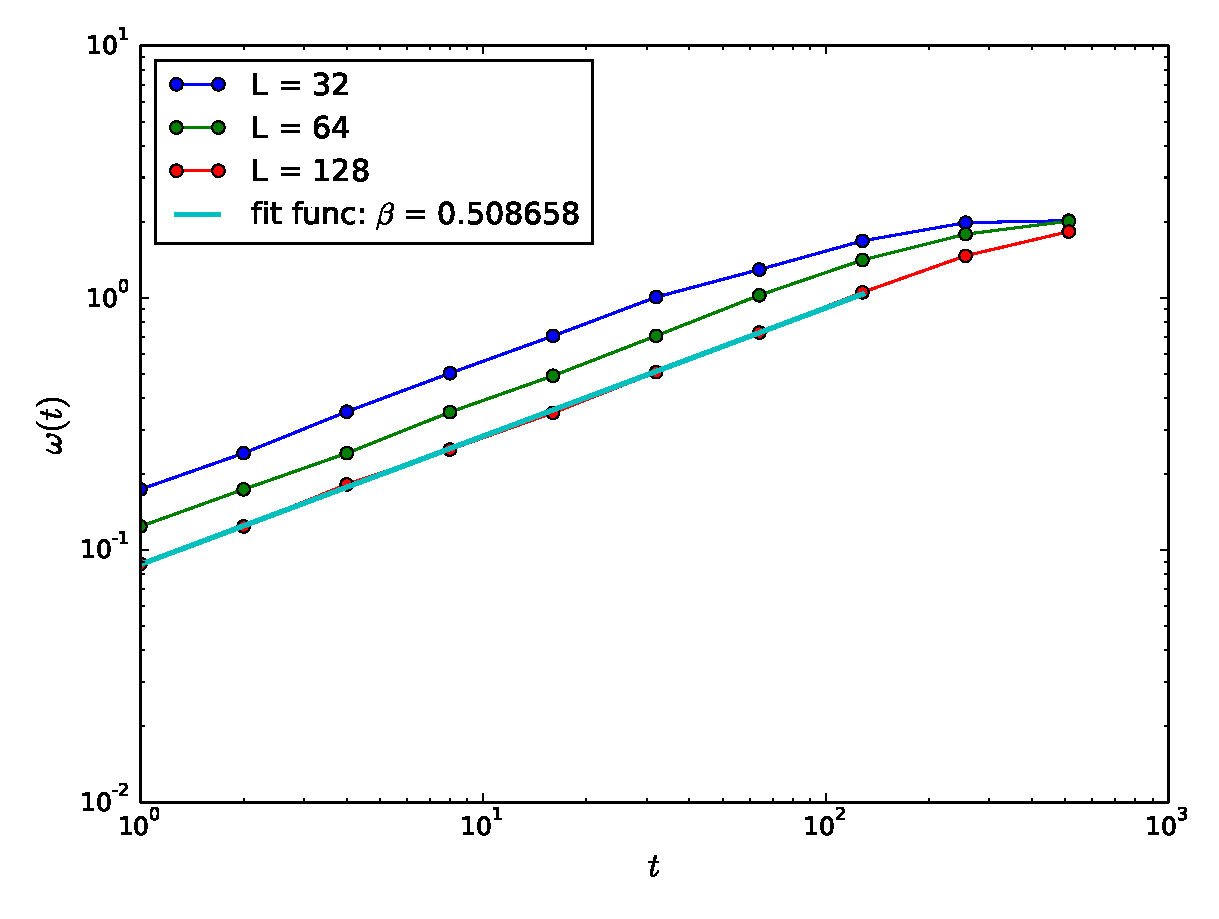
\includegraphics[width=10.0cm]{figure_3.pdf}
                        \caption{$L=32,64,128$について幅$\omega(t)$を時間$t$の関数として両対数グラフにしたもの($T \sim 1000$).直線の傾きが$\beta$を表す.}
                        \label{fig:14-12-f3}
                    \end{center}
                \end{figure}
                
                また,$t$の十分大きいところでは,それぞれの$L$に対してグラフは水平になり,それ以上変化しないようになる.このような状況になったときの$L$に対する$\omega$の値を比較すれば,
                
                \begin{equation}
                    \omega(L, t \gg 1) \sim L^{\alpha}
                \end{equation}
                の式から$\alpha$を求めることができる.
                
                図\ref{fig:14-12-f2}から,$L$が大きいほど,表面の幅が定常状態の値となるクロスオーバー時間は長くなるので,計算量を少なくしながらも,できるだけ正確な$\alpha$の値を得るためには,100程度までの$L$について,それぞれの$\omega$の定常状態の値を測定し,それらを一つのグラフに横軸$L$,縦軸$\omega$の両対数グラフにして,その傾きを求めれば良い.このようにして得られた$L$に対する$\omega$のグラフを図\ref{fig:14-12-f4}に示す.このグラフは直線で近似することができ,その傾き$\alpha$は図に示す通りであった.ただし,この値も$\alpha=1/2$とは異なっているように思われる.
                
                \begin{figure}[H]
                    \begin{center}
                        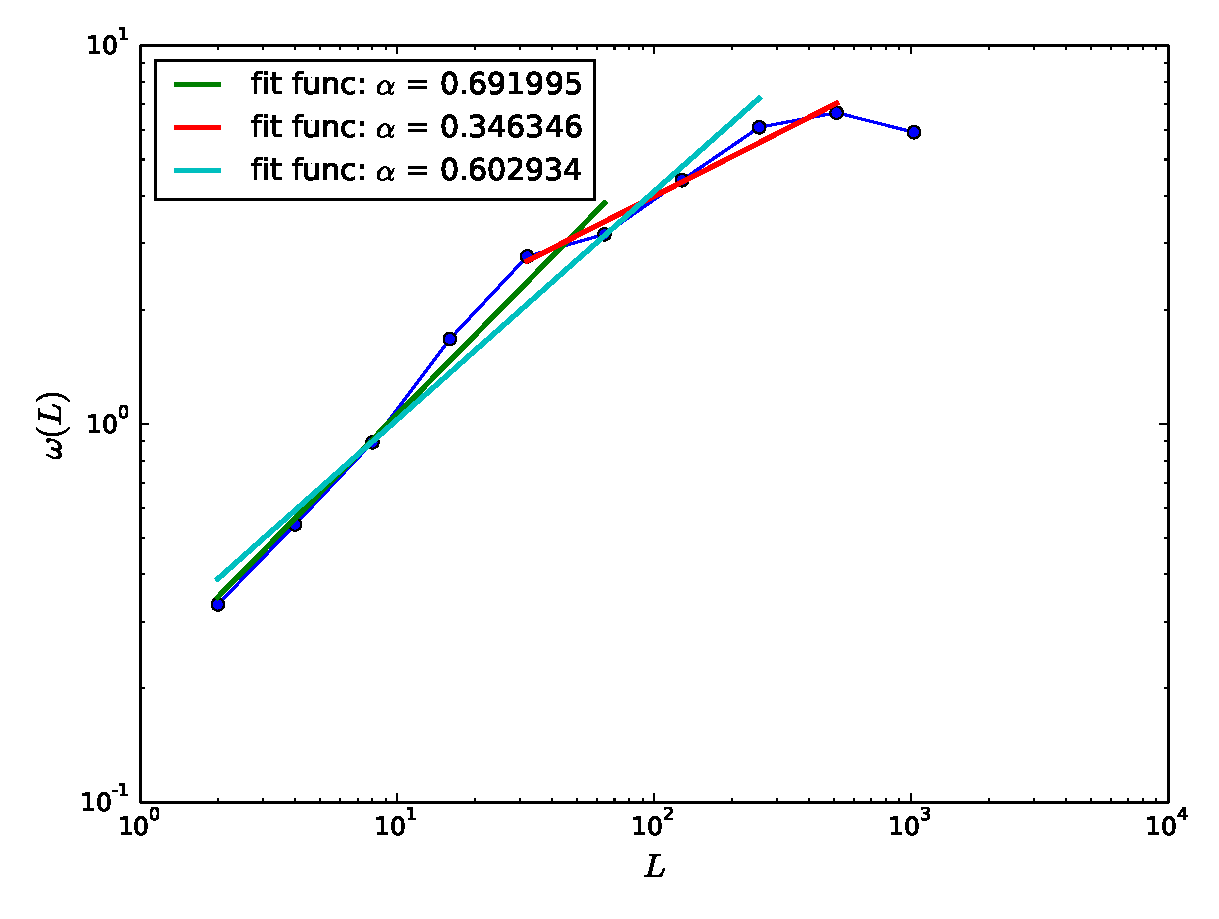
\includegraphics[width=10.0cm]{figure_4.pdf}
                        \caption{$L=32,64,128$について幅$\omega(t)$を時間$t$の関数として両対数グラフにしたもの($T \sim 1000$).直線の傾きが$\beta$を表す}
                        \label{fig:14-12-f4}
                    \end{center}
                \end{figure}
                
            \end{enumerate}
        
        \item $\omega(L,t)$および$L$依存性は,スケーリング仮設
        \begin{equation}
            \omega(\varepsilon^{a}L, \varepsilon^{b}t) = \varepsilon^{c}\omega(L,t)
        \end{equation}
        をたてることにより,$\varepsilon^{a}L=1$とおくと
        \begin{equation}
            \varepsilon = L^{-1/a}
        \end{equation}
        であり,これを代入すると,
        \begin{equation}
            \omega(1, L^{-b/a}t) \equiv f(t/L^{b/a}) = L^{-c/a}\omega(L,t)
        \end{equation}
        のようにスケーリング関数$f$を決定することができ,$\alpha=c/a, \beta=c/b$とおくと,
        \begin{equation}
            \omega(L, t) \approx L^{\alpha}f(t/L^{\alpha/\beta})
            \label{eq:14-12-e1}
        \end{equation}
        で表すことができる.ここで,
        \begin{eqnarray}
            f(x) \approx x^{\beta},\ \  x \ll 1 の場合\\
            f(x) = 一定,\ \  x \gg 1 の場合
        \end{eqnarray}
        である.設問bで考えられた$L$のいろいろな値について,比$\omega(L,t)/L^{\alpha}$を$t/L^{\alpha / \beta}$に対してプロットすることにより,スケーリングの形(\ref{eq:14-12-e1})の存在を確認せよ.このスケーリング式が成り立つならば,異なる$L$の値に対する$\omega$の結果は普遍的な曲線上にのる.設問bで得られた$\alpha$,$\beta$の値,または正確な値を用いよ.
            \begin{enumerate}
                \item 以下の図\ref{fig:14-12-f5}に示すように,様々な$L$に対して,時間$t$と表面の幅$\omega(L,t)$の関係を,横軸を$t/L^{\alpha/\beta}$,縦軸を$\omega(L,t)/L^{\alpha}$として両対数グラフにすると,1つの曲線にまとめられることが見て取れる.
                \begin{figure}[H]
                    \begin{center}
                        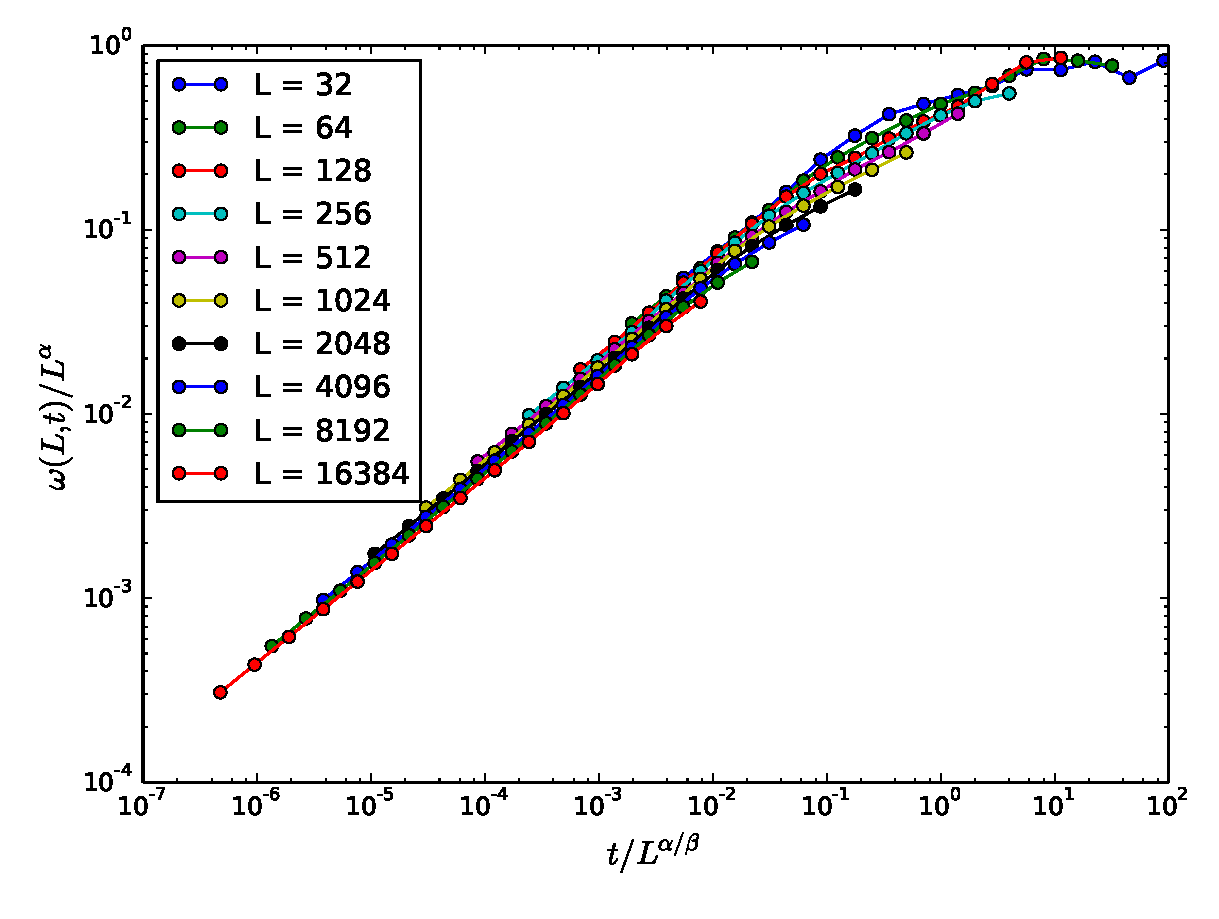
\includegraphics[width=10.0cm]{figure_5.pdf}
                        \caption{様々な$L$に対し,横軸を$t/L^{\alpha/\beta}$,縦軸を$\omega(L,t)/L^{\alpha}$として両対数グラフにた.スケーリングの関係(\ref{eq:14-12-e1})の存在を確認できる.}
                        \label{fig:14-12-f5}
                    \end{center}
                \end{figure}
            \end{enumerate}
        
    \end{enumerate}

\section{まとめ}
    成長する表面を,イーデンモデルによるシミュレーションで考えることができ,そのときの表面の幅$\omega$の性質について考えることができた.指数の値が期待している値とならないことが不思議ではあるが,現段階で間違いを見つけることができなかった.
\nocite{textbook}
\nocite{fractal1}
\bibliography{/home/shotaro/Workspace/computing_simulation/reference}


\end{document}
